\PassOptionsToPackage{svgnames}{xcolor}
\documentclass[a4paper, 12pt]{article}

\usepackage{hyperref}
\usepackage{pgf-pie}
\usepackage{subfiles}

\hypersetup{
	colorlinks,
	linkcolor={black},
	citecolor={black},
	urlcolor={black}
}
\usepackage{lmodern}
%\usepackage{geometry}
%\usepackage{layout}
\usepackage{graphicx}
\usepackage{wrapfig}

\title{Artificial Teacher}
\author{Alex Tsvetanov}	

\newcommand{\titleGP}{\begingroup
	\centering
	%\vspace{\baselineskip}
	\rule{\textwidth}{1.6pt}\vspace{-\baselineskip}\vspace{2pt}
	\rule{\textwidth}{0.4pt}\\[\baselineskip]
	
	{\LARGE Robosapien - the AI traveler \\ \small{Towards Future Society 5.0: Modeling, Exploration \& Understanding}}\\[0.2\baselineskip]
	
	\rule{\textwidth}{0.4pt}\vspace{-\baselineskip}\vspace{3.2pt}
	\rule{\textwidth}{1.6pt}\\[\baselineskip]
	%\begin{wrapfigure}{l}{0.35\textwidth}
		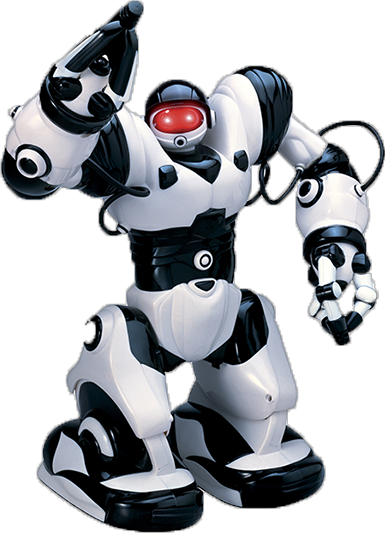
\includegraphics[width=0.35\textwidth]{robot.png}
	%\end{wrapfigure}
	
	\vspace{50pt}
	{
	{\LARGE Alex Tsvetanov}\\
	{\normalsize Sofia High School of Mathematics, Sofia, Bulgaria}\\\vspace{0.5cm} \& \vspace{0.5cm} \\
	{\LARGE Ivaylo Ivanov}\\
	{\normalsize High School of Natural Sciences and Mathematics, Stara Zagora, Bulgaria}\par}
	
	\vspace{2\baselineskip}
	
	{\scshape \large
		Under the direction of \\
		\hspace{-0.3cm}\href{https://bg.linkedin.com/in/zlatogor-minchev-a101b85}{Assoc. Prof. Zlatogor Minchev} \\\par
	}
	\vspace{1cm}
	
	
	\vfill
	
	{\scshape Summer Research School, Aug 2018} \\[0.3\baselineskip]
	{\large Pamporovo, Bulgaria }\par
	
	\endgroup}

\usepackage{tcolorbox}
\newenvironment{myblock}[1]{%
	\tcolorbox[beamer,%
	noparskip,breakable,
	colback=LightGreen,colframe=DarkGreen,%
	colbacklower=LimeGreen!75!LightGreen,%
	title=#1]}%
{\endtcolorbox}
\newenvironment{myblocksecond}[1]{%
	\tcolorbox[beamer,%
	noparskip,breakable,
	colback=Yellow,colframe=Brown,%
	colbacklower=Brown!75!Yellow,%
	title=#1]}%
{\endtcolorbox}

\begin{document}
	
	\titleGP
	\newpage
	
	\tableofcontents
	\newpage
	
	\begin{abstract}
		Today's robots excel at performing pre-programmed tasks. They work well in
		highly controlled environments with well-defined objects. Artificial Intelligence
		and Robotics have a common root and a (relatively) long history of interactions
		and scientific discussions. The birth of Artificial Intelligence and Robotics takes
		place in the same period ('50), and initially there was no clear distinction
		between the two disciplines. Dreams like exoskeletons and robots controlled
		remotely with an interactive humanoid interface are already a reality. \\
		
		Robosapiens is a robot that allows us to perform tasks such as a Martian surface
		exploration using a mixed reality.\\
		
		The core aim of this project is to introduce the capabilities of a robo-researcher with
		his new capabilities to overcome various obstacles without the help of a user to
		manage it.\\
		
		By developing this project, we hope to reduce the lifetime to Society 5.0 and to live in a smarter and easier world. \\
		
		Tomorrow's robots will create increasingly rich maps of the real world and the
		objects in it and they will do so in human terms, allowing for a new level of human-robot interaction.
	\end{abstract}
	\newpage
	
	\section{Introduction}
	\subfile{introduction}
	\section{Implementation}
	\subfile{implementation}
	\section{Acknowledgments}
	Special thanks to:
	\begin{itemize}
		\item Zlatogor Minchev for helping us to set up the hardware
	\end{itemize}
	Thanks also to:
	\begin{itemize}
		\item High School Students Institute of Mathematics and Informatics
		\item Bulgarian Academy of Sciences
	\end{itemize}
	\begin{thebibliography}{99}
		\bibitem{robosapientopstrickshacks}
		{\itshape The Robosapien Companion: Tips, Tricks, and Hacks}.\\
		Copyright $\copyright$ 2005 Jamie Samans\\
		\bibitem{aistuartandpeter}
		{\itshape Artificial Intelligence: A Modern Approach - third edition}\\
		Stuart J. Russell and Peter Norvig\\
		
		\bibitem{opencv}
		{\itshape Open Source Computer Vision Library}\\
		\texttt{https://github.com/opencv/opencv} \\
		
		\bibitem{tensorflow}
		{\itshape TensorFlow}\\
		\texttt{Copyright $\copyright$ 2018 The TensorFlow Authors.} \\
		
		\bibitem{keras}
		{\itshape Keras}\\
		\texttt{https://github.com/keras-team/keras/} \\
		
		\bibitem{sbar}
		{\itshape The ZBar QR Code reader} \\
		\texttt{Copyright $\copyright$ 1999-2009 Timothy B. Terriberry} \\
		
		\bibitem{gcc}
		{\itshape GNU Compiler Collection}.
		\texttt{https://gcc.gnu.org/}. \\
		Copyright $\copyright$  2009 Free Software Foundation, Inc. \\
		
		\bibitem{latex}
		{\itshape \LaTeX}.\\
		\texttt{https://www.latex-project.org/}.
	\end{thebibliography}
\end{document}
